\documentclass[10pt,t,english,aspectratio=1610]{beamer}
\usepackage{fontawesome}
\usepackage{graphicx}
\usepackage{array}
\usepackage[normalem]{ulem}
\usepackage{amsfonts,amsmath,amssymb,bm,bbm}
\usepackage{mathrsfs}
% NOTE: sgame is intentionally NOT used -- its `game` environment is
% incompatible with the `array` package (required by colortbl/makecell/multirow)
% and errors with "Missing # inserted in alignment preamble". We use the modern
% TikZ-based `xgames` package instead (loaded after TikZ below).
\usepackage{graphicx,pstricks}
\usepackage{xcolor}
\usepackage{colortbl}
\usepackage{makecell}
\usepackage{tikz,tikzsymbols,gnuplottex}
\usetikzlibrary{decorations.pathreplacing,shapes,positioning,arrows.meta,fit,backgrounds,calc}

% --- xgames: TikZ-based game-theory typesetting (matrixgame, gametree,
% beliefspace, automaton). Not on CTAN; xgames.sty + fikz.sty are vendored at
% the repo root. CC BY-SA 4.0 (xgames) / GPL-3.0 (fikz), (c) Benjamin Bernard.
\usepackage{xgames}

% Custom command for shading rows in a matrixgame
% ---------------------------------------------------------------------------
% \shaderow[<fill options>]{<row>}{<first column>}{<last column>}
% Call this inside the matrixgame, after \payoffmatrix
% Can wrap in a \foreach to shade multiple regions
% Example: \foreach \i in {1,...,5}{ \shaderow[green!50!black]{\i}{\i}{5} }
\newcommand{\shaderow}[4][red!60]{%
  \ifnum#3=1\relax\def\xl{0}\else\pgfmathsetmacro{\xl}{\pmtwi[#3-1]}\fi
  \ifnum#2=1\relax\def\yt{0}\else\pgfmathsetmacro{\yt}{\pmthi[#2-1]}\fi
  \pgfmathsetmacro{\xr}{\pmtwi[#4]}%
  \pgfmathsetmacro{\yb}{\pmthi[#2]}%
  \fill[opacity=0.18, #1] ($(pmt1-tl)+(\xl,-\yt)$) rectangle ($(pmt1-tl)+(\xr,-\yb)$);%
}

\usepackage[english]{babel}
\usepackage[utf8]{inputenc}
\usepackage{appendixnumberbeamer}
\usepackage{datetime2}
\usepackage{booktabs}
\usepackage{setspace}
\usepackage{rotating}
\usepackage{multirow}
\usepackage{listings}

\usepackage{natbib}
\bibliographystyle{unsrtnat}
\renewcommand{\bibfont}{\footnotesize}
\renewcommand{\bibsection}{\vspace{-1em}}

%\usepackage{matlab-prettifier} % For enhanced MATLAB highlighting
\lstset{
    language=matlab,
    % Other options for styling (optional)
    basicstyle=\ttfamily\footnotesize, % Font style
    keywordstyle=\color{blue}, % Keyword color
    commentstyle=\color{green!50!black}, % Comment color
    stringstyle=\color{red!70!black}, % String color
    numbers=left, % Line numbers on the left
    numberstyle=\tiny\color{gray}, % Style for line numbers
    frame=single, % Frame around the listing
    breaklines=true, % Allow line breaking
    captionpos=b, % Caption at the bottom
    tabsize=4 % Tab size
}

% ------------------------------------------------------------------------------
% Use the beautiful metropolis beamer template
% ------------------------------------------------------------------------------
\usepackage[T1]{fontenc}
\usepackage[utf8]{inputenc}
\usepackage{fontawesome}
\usepackage{FiraSans} 
\mode<presentation>
{
  \usetheme[progressbar=foot,background=light]{metropolis} 
  \usecolortheme{default} % or try albatross, beaver, crane, ...
  \usefonttheme{default}  % or try default, serif, structurebold, ...
  \setbeamertemplate{navigation symbols}{}
  \setbeamertemplate{caption}[numbered]
  %\setbeamertemplate{frame footer}{My custom footer}
  \makeatletter
    \setbeamertemplate{frametitle continuation}{}
  \makeatother
} 
\addtobeamertemplate{frametitle continuation}{}{%
  \setbeamertemplate{frametitle continuation}{}%
}
\setbeamertemplate{frametitle continuation}{}

\newenvironment{stepenumerate}{\begin{enumerate}[<+->]}{\end{enumerate}}
\newenvironment{stepitemize}{\begin{itemize}[<+->]}{\end{itemize} }
\newenvironment{stepenumeratewithalert}{\begin{enumerate}[<+-| alert@+>]}{\end{enumerate}}
\newenvironment{stepitemizewithalert}{\begin{itemize}[<+-| alert@+>]}{\end{itemize} }

\newtheorem{question}{Question}
\newtheorem{claim}{Claim}
\newtheorem{proposition}{Proposition}
\newtheorem{remark}{Remark}
\newtheorem{conjecture}{Conjecture}

\definecolor{metrop}{RGB}{29, 44, 44}
\colorlet{GrayLight}{black!15}
\colorlet{GrayMedium}{black!30}
\colorlet{ForestGreen}{green!60!black}

\newenvironment{transitionframe}{
  \setbeamercolor{background canvas}{bg=black!80}
  \begin{frame}}{
    \end{frame}
}

\newcommand{\bsk}{

\bigskip

}

\newcommand{\pd}{\partial}
\newcommand{\RR}{\mathbb{R}}

\newcommand*\hugme[1]{\tikz[baseline=(char.base)]{\node[shape=ellipse,draw,inner sep=0pt] (char) {#1};}}

\newcounter{saveenumi}
\newcommand{\seti}{\setcounter{saveenumi}{\value{enumi}}}
\newcommand{\conti}{\setcounter{enumi}{\value{saveenumi}}}
\resetcounteronoverlays{saveenumi}



\newcommand\dotprod[2]{\langle #1 , #2 \rangle}
\newcommand{\ft}[1]{\widehat #1}
\newcommand{\qabove}[1]{\overset{\text{\large \textbf ?}}{#1}}
\newcommand{\eqae}{\overset{\text{a.e.}}{=}}
\newcommand{\calp}{\mathcal{P}}
\newcommand{\calg}{\mathcal{G}}
\newcommand{\calb}{\mathcal{B}}
\newcommand{\textd}{\text{d}}
\newcommand{\bbr}{\mathbb{R}}
\newcommand{\binm}{\mathbin{M}}
\newcommand{\binc}{\mathbin{C}}
\newcommand{\binb}{\mathbin{B}}
\newcommand{\calc}{\mathcal{C}}
\newcommand{\calh}{\mathcal{H}}
\newcommand{\bfone}{\mathbf{1}}
\newcommand{\bbe}{\mathbb{E}}
\newcommand{\bfle}{\mathbf{e}}
\newcommand{\calf}{\mathcal{F}}
\newcommand{\cala}{\mathcal{A}}
\newcommand{\cale}{\mathcal{E}}
\newcommand{\bbn}{\mathbb{N}}
\newcommand{\cantor}{\calc}
\newcommand{\calY}{\mathcal{Y}}
\newcommand{\textb}{\text{B}}
\newcommand{\calm}{\mathcal{M}}
\newcommand{\bint}{\mathbin{T}}
\newcommand{\ep}{\epsilon}
\newcommand{\bbq}{\mathbb{Q}}
\newcommand{\bbp}{\mathbb{P}}
\newcommand{\cals}{\mathcal{S}}
\newcommand{\emptysequence}{e}
\newcommand{\bbz}{\mathbb{Z}}
\newcommand{\fraka}{\frak{A}}
\newcommand{\frakb}{\frak{B}}
\newcommand{\length}{\text{length}}
\newcommand{\bfn}{\mathbf{N}}
\newcommand{\support}{\text{support}}
\DeclareMathOperator*{\argmax}{arg\,max}
\newcommand{\dom}{\mbox{dom}}
\def\ut{\underline t}
\def\um{\underline m}
\def\PP{\mathbb{P}}
\def\EE{\mathbb{E}}
\def\RR{\mathbb{R}}

% Title page info
\title[Behavioral Strategies]{Chapter 7: Behavioral Strategies}
\author[ECON 5001]{ECON 5001\\Prof. Paul J. Healy\\Based on: \textit{Game Theory} by Giacomo Bonanno} \color{metrop}
\institute[OSU]{}
\date[]{\vfill {\tiny Updated \today\ at\ \DTMcurrenttime}}

% ---------------------------------------------------------------------
% SCOPE AND NOTATION
%   Same as decks 07-08: u(o) = outcome utility, U(L) = expected utility,
%   pi_i = payoff at a pure profile, Pi_i = expected payoff at a mixed one.
%   Section 7.1's formal "cardinal extensive-form game" (vNM ranking of
%   L(O) attached to a frame) is NOT taught. Same rule as deck 08: a
%   lottery (or a Nature node) at the end of a branch gets replaced by its
%   expected utility. Nothing later depends on more.
%   Bonanno's Figs 7.1-7.6 example is replaced by the running Ohio State
%   vs. Michigan example. Fig 7.4 (no perfect recall), Fig 7.7 (three-player
%   SPNE) and Fig 7.12 (Selten's horse) are the book's own.
%   Behavioral profiles are written Bonanno's way: one matrix per player,
%   a vertical bar between that player's information sets.
%
% ANSWERS (all checked numerically)
%   Last play: OSU down 1 after a TD, no time left. u(Win)=100, u(Lose)=0
%   for OSU; Michigan gets 100 minus that. Kick: good .95, then overtime
%   is a 50-50 coin flip. Go for 2: deck 08's Run/Pass table.
%     Overtime node -> (50,50). Kick -> .95(50) + .05(0) = 47.5 -> (47.5, 52.5)
%     Subgame: no pure NE. Mixed NE OSU Run 3/5, Michigan Stop Run 1/2,
%       payoffs (60,40). OSU goes for 2 (60 > 47.5).
%     SPNE: OSU (Kick 0, Go 1 | Run 3/5, Pass 2/5), Michigan (SR 1/2, SP 1/2)
%   OSU has 4 pure strategies (KR, KP, GR, GP): mixed needs 3 numbers,
%     behavioral needs 2. Michigan has one infoset: mixed = behavioral.
%   Mixed (KR .1, KP .3, GR .36, GP .24) -> behavioral (Go .6 | Run .6).
%     KR/KP split doesn't matter. Vs Michigan's NE mix it earns 55.
%   Counting: 3 infosets x 2 choices -> 8 pure, mixed 7, behavioral 3
%   Fig 7.4: (a,c) 1/2, (b,d) 1/2 gives z1 1/2, z4 1/2. Behavioral (p, q):
%     P(z2) = p(1-q) = 0 forces p=0 (so P(z1)=0) or q=1 (so P(z4)=0)
%   Fig 7.7: left subgame P2 (A 1/2), P3 (C 1/4), payoffs (1.125,.75,2)
%     right subgame P2 (E 2/3), P3 (G 1/3), payoffs (1, .67, 2.33)
%     P1 picks L. SPNE (L | A 1/2 | E 2/3 | C 1/4 | G 1/3)
%   Selten's horse: no proper subgames, SPNE = NE. Pure NE (a,e,c),
%     (a,f,c), (b,e,c) all pay (2,2,2); (b,f,d) pays (1,1,0).
%     Bonanno p. 249 says "Player 1 plays a" for (b,f,d); should be b.
%   Gameday parking 2 (deck 08's parking game is the subgame):
%     Jordan 6 pure strategies (Bus/Drive x Pay/West/Neil). Mixed 5,
%     behavioral 3. CampusParc one infoset.
%     Bus: on time 3/4 -> 2, late 1/4 -> 0. EU 1.5. CampusParc 0.
%     Subgame NE: Jordan (0, 1/3, 2/3), CampusParc (PW 4/7, PN 3/7),
%     payoffs (12/7, 2/3). 12/7 = 1.71 > 1.5 -> Drive.
%     SPNE: Jordan (Bus 0, Drive 1 | Pay 0, West 1/3, Neil 2/3),
%           CampusParc (PW 4/7, PN 3/7)
%     Bus worth it if 2r >= 12/7, i.e. on-time chance r >= 6/7 (86%)
% ---------------------------------------------------------------------

% Behavioral strategy: \beh{choices}{probabilities}, rows separated by &,
% column spec given as optional arg, e.g. \beh[cc|cc]{a & b & e & f}{...}
\newcommand{\beh}[3][cc]{\left(\begin{array}{#1} #2 \\ #3 \end{array}\right)}

% Same tree, drawn several times: the last play of the game
\newcommand{\lastplaytree}[1][0.78]{%
\begin{gametree}[player names={OSU, Michigan}, scale=#1]
  \branch[player=1, root=w, label=90] from (0,0) to[v=1.25, h=7.4] {Kick; Go for 2};
  \branch[player=0, label=150] from (w1) to[v=1.35, h=3.2] {Good\ $.95$; Miss\ $.05$(0,100)};
  \branch[player=0, label=150, label text=OT] from (w11) to[v=1.35, h=2.0] {Win\ $\frac12$(100,0); Lose\ $\frac12$(0,100)};
  \branch[player=1, label=0] from (w2) to[v=1.35, h=3.6] {Run; Pass};
  \branch[player=2, label=none] from (w21) to[v=1.6, h=1.75] {SR(40,60); SP(80,20)};
  \branch[label=none] from (w22) to {SR(90,10); SP(30,70)};
  \informset (w21) -- (w22);
  \path (-6.4,0.5) rectangle (7.0,-4.9);
\end{gametree}}

% Bonanno Figure 7.7
\newcommand{\figsevenseven}{%
  \branch[player=1, root=w, label=90] from (0,0) to[v=1.1, h=7.6] {L; R};
  \branch[player=2, label=135] from (w1) to[v=1.2, h=3.0] {A; B};
  \branch[player=3, label=none] from (w11) to[v=1.35, h=1.35] {C(1,3,1); D(2,0,2)};
  \branch[label=none] from (w12) to {C(2,0,3); D(0,1,2)};
  \informset[player=3] (w11) -- (w12);
  \branch[player=2, label=45] from (w2) to[v=1.2, h=3.0] {E; F};
  \branch[player=3, label=none] from (w21) to[v=1.35, h=1.35] {G(2,0,3); H(0,1,2)};
  \branch[label=none] from (w22) to {G(1,2,1); H(2,0,3)};
  \informset[player=3] (w21) -- (w22);
}

% Selten's horse (Bonanno Figure 7.12), drawn by hand: xgames trees only
% grow downward, and the horse's top row is horizontal
\newcommand{\horse}[1][]{%
\begin{tikzpicture}[>=Stealth, scale=0.95,
    dot/.style={circle, fill, inner sep=1.7pt},
    pay/.style={align=center, font=\small, inner sep=1pt}]
  \node[dot] (n1) at (0,0) {};
  \node[dot] (n2) at (3.2,0) {};
  \node[dot] (t)  at (5.8,0) {};
  \node[dot] (x)  at (0,-1.9) {};
  \node[dot] (y)  at (3.2,-1.9) {};
  \node[font=\large, text=player1, above=3pt] at (n1) {1};
  \node[font=\large, text=player2, above=3pt] at (n2) {2};
  \draw[->, thick] (n1) -- node[above] {$b$} (n2);
  \draw[->, thick] (n2) -- node[above] {$f$} (t);
  \draw[->, thick] (n1) -- node[left] {$a$} (x);
  \draw[->, thick] (n2) -- node[left] {$e$} (y);
  \node[pay, right=3pt] at (t.east) {\textcolor{player1}{1}\\\textcolor{player2}{1}\\\textcolor{player3}{0}};
  \draw[thick, rounded corners=7pt, player3] ($(x)+(-0.4,0.3)$) rectangle ($(y)+(0.4,-0.3)$);
  \node[font=\large, text=player3] at ($(x)!0.5!(y)$) {3};
  \foreach \n/\s in {x/0, y/3.2}{
    \node[dot] (\n c) at (\s-0.7,-3.5) {};
    \node[dot] (\n d) at (\s+0.7,-3.5) {};
    \draw[->, thick] (\n) -- node[left] {$c$} (\n c);
    \draw[->, thick] (\n) -- node[right] {$d$} (\n d);
    \node[pay, below=2pt] at (\n c.south) {\textcolor{player1}{2}\\\textcolor{player2}{2}\\\textcolor{player3}{2}};
    \node[pay, below=2pt] at (\n d.south) {\textcolor{player1}{0}\\\textcolor{player2}{0}\\\textcolor{player3}{0}};
  }
  #1
\end{tikzpicture}}

\begin{document}

\frame{\maketitle}

\begin{frame}{Where We Left Off}
Chapter 4: game trees with \textbf{information sets}, solved by SPNE
\begin{itemize}
    \item Solve the smallest subgames first, replace, repeat
    \item Problem: a subgame might have \textbf{no} NE $\Rightarrow$ no SPNE!
\end{itemize}
\bsk
Chapter 6: \textbf{mixed strategies}
\begin{itemize}
    \item Nash: every finite game has a (mixed) NE
\end{itemize}
\vfill
Our goal:
\begin{enumerate}
    \item Put lotteries and mixing into game trees
    \item Find a \textbf{simpler} way to mix in trees: behavioral strategies
    \item Show that a SPNE always exists
    \item See what SPNE still gets wrong
\end{enumerate}
\vspace{-0.4in}
\end{frame}

% ==============================================================
% RUNNING EXAMPLE: THE LAST PLAY
% ==============================================================

\begin{frame}[standout]
Lotteries in Game Trees
\end{frame}

\begin{frame}{The Last Play of The Game}
Ohio State at Michigan. OSU scores a touchdown as time runs out
\begin{itemize}
    \item Now down by \textbf{1}. One more play
\end{itemize}
\bsk
OSU chooses:
\begin{itemize}
    \item \textbf{Kick} the extra point. Good 95\% of the time $\Rightarrow$ tie $\Rightarrow$ overtime
    \begin{itemize}
        \item Overtime: call it a 50-50 coin flip
    \end{itemize}
    \item \textbf{Go for 2}. Then the Chapter 6 game:
    \begin{itemize}
        \item OSU: \textbf{Run} or \textbf{Pass}
        \item Michigan (doesn't see OSU's call): \textbf{Stop Run (SR)} or \textbf{Stop Pass (SP)}
    \end{itemize}
\end{itemize}
\bsk
Payoffs: \ $u(\text{Win})=100$, $u(\text{Lose})=0$ for OSU. Michigan: the opposite
\vfill
{\footnotesize Hypothetical numbers. Two-point success rates are the same as Chapter 6.}
\vspace{-0.2in}
\end{frame}

\begin{frame}{Draw It}
\centering
\only<1>{\begin{gametree}[player names={OSU, Michigan}, scale=0.78]
  \branch[player=1, root=w, label=90] from (0,0) to[v=1.25, h=7.4] {Kick; Go for 2};
  \path (-6.4,0.5) rectangle (7.0,-4.9);
\end{gametree}}%
\only<2>{\begin{gametree}[player names={OSU, Michigan}, scale=0.78]
  \branch[player=1, root=w, label=90] from (0,0) to[v=1.25, h=7.4] {Kick; Go for 2};
  \branch[player=0, label=150] from (w1) to[v=1.35, h=3.2] {Good\ $.95$; Miss\ $.05$(0,100)};
  \branch[player=0, label=150, label text=OT] from (w11) to[v=1.35, h=2.0] {Win\ $\frac12$(100,0); Lose\ $\frac12$(0,100)};
  \path (-6.4,0.5) rectangle (7.0,-4.9);
\end{gametree}}%
\only<3->{\lastplaytree}
\bsk
\raggedright
\only<1>{OSU moves first}%
\only<2>{Kick: two moves by Nature. Each branch has a probability}%
\only<3>{Go for 2: a simultaneous-move game hanging off the tree}%
\only<4>{How many proper subgames? \underline{\hspace{0.6in}}}
\vspace{-0.2in}
\end{frame}

\begin{frame}{Nature Gives a Lottery}
\begin{columns}[T]
\begin{column}{0.45\textwidth}
\centering
After OSU chooses Kick:
\bsk
\begin{gametree}[player names={OSU, Michigan}, scale=0.85]
  \branch[player=0, root=w, label=90] from (0,0) to[v=1.4, h=3.6] {Good\ $.95$; Miss\ $.05$(0,100)};
  \branch[player=0, label=150, label text=OT] from (w1) to[v=1.4, h=2.4] {Win\ $\frac12$(100,0); Lose\ $\frac12$(0,100)};
\end{gametree}
\end{column}
\begin{column}{0.53\textwidth}
Overtime gives OSU
$\begin{pmatrix} \text{Win} & \text{Lose} \\ \tfrac12 & \tfrac12\end{pmatrix}$
\bsk
$U(\text{OT})=$ \underline{\hspace{1in}}
\bsk
Kick gives OSU
$\begin{pmatrix} \text{OT} & \text{Lose} \\ .95 & .05\end{pmatrix}$
\bsk
$U(\text{Kick})=$ \underline{\hspace{1in}}
\end{column}
\end{columns}
\bsk
\textbf{Rule:} Same as Chapter 6. A lottery at the end of a branch? Use its expected utility
\bsk
\onslide<2->{So: replace the whole Kick branch with \underline{\hspace{0.9in}}}
\vfill
{\footnotesize Bonanno (\S7.1) also writes the lottery right at the terminal node instead of drawing Nature. Same thing.}
\vspace{-0.2in}
\end{frame}

% ==============================================================
% 7.2 SUBGAME-PERFECT EQUILIBRIUM REVISITED
% ==============================================================

\begin{frame}[standout]
Subgame-Perfect Equilibrium, Revisited
\end{frame}

\begin{frame}{Step 1: Solve the Subgame}
\begin{columns}[c]
\begin{column}{0.45\textwidth}
\centering
\begin{gametree}[player names={OSU, Michigan}, scale=0.78]
  \branch[player=1, root=w, label=90] from (0,0) to[v=1.35, h=3.6] {Run; Pass};
  \branch[player=2, label=none] from (w1) to[v=1.35, h=1.75] {SR(40,60); SP(80,20)};
  \branch[label=none] from (w2) to {SR(90,10); SP(30,70)};
  \informset (w1) -- (w2);
\end{gametree}
\end{column}
\begin{column}{0.53\textwidth}
\centering
\begin{matrixgame}[top={Stop Run, Stop Pass}, left={Run, Pass}, player names={OSU, Michigan}, w=1.9, br=<2->]
  \payoffmatrix{40,60 & 80,20 \\ 90,10 & 30,70}
\end{matrixgame}
\end{column}
\end{columns}
\bsk
\onslide<2->{No pure NE. \ Chapter 4 (ordinal payoffs): algorithm \textbf{halts}. No SPNE!\\}
\onslide<3->{Chapter 6 (cardinal payoffs): mixed NE. \ OSU Run \underline{\hspace{0.5in}}, \ Michigan Stop Run \underline{\hspace{0.5in}}\\[6pt]
Payoffs: \ (\underline{\hspace{0.45in}}, \underline{\hspace{0.45in}})}
\vspace{-0.3in}
\end{frame}

\begin{frame}{Step 2: Replace and Solve}
\centering
\begin{gametree}[player names={OSU, Michigan}, scale=1.0]
  \branch[player=1, root=w, label=90] from (0,0) to[v=1.6, h=6.0] {Kick(47.5,52.5); Go for 2(60,40)};
\end{gametree}
\bsk
\raggedright
Kick: Nature's lottery, replaced by its expected utility\\
Go for 2: the subgame, replaced by its \textbf{mixed} NE payoffs
\bsk
OSU chooses: \underline{\hspace{1in}}
\vfill
\onslide<2->{Real coaches carry a chart for exactly this decision}
\vspace{-0.3in}
\end{frame}

\begin{frame}{The SPNE}
Write a probability at \textbf{every} decision point:
\bsk
\centering
OSU: \ $\beh[cc|cc]{\text{Kick} & \text{Go} & \text{Run} & \text{Pass}}{\underline{\hspace{0.3in}} & \underline{\hspace{0.3in}} & \underline{\hspace{0.3in}} & \underline{\hspace{0.3in}}}$
\qquad
Michigan: \ $\beh{\text{SR} & \text{SP}}{\underline{\hspace{0.3in}} & \underline{\hspace{0.3in}}}$
\bsk
\raggedright
\only<2->{\textbf{Notice:} we didn't write a probability for each \textbf{strategy}\\
We wrote one probability distribution per \textbf{information set}\\}
\only<3->{\bsk That's called a \textbf{behavioral strategy}}
\vspace{-0.3in}
\end{frame}

\begin{frame}{Selten's Theorem}
\begin{block}{Theorem (Selten, 1965)}
Every finite extensive-form game with cardinal payoffs has \textbf{at least one} SPNE in mixed strategies
\end{block}
\bsk
Why?
\begin{itemize}
    \item Every subgame is a finite game
    \item Nash: every finite game has a (mixed) NE
    \item So the SPNE algorithm \textbf{never halts}
\end{itemize}
\bsk
Ordinal payoffs: SPNE might not exist\\
Cardinal payoffs: SPNE always exists
\vfill
{\footnotesize Reinhard Selten shared the 1994 Nobel Prize with John Nash and John Harsanyi.}
\vspace{-0.2in}
\end{frame}

% ==============================================================
% 7.1 BEHAVIORAL STRATEGIES
% ==============================================================

\begin{frame}[standout]
Behavioral Strategies
\end{frame}

\begin{frame}{OSU's Strategies}
A strategy: one choice at every information set (Chapter 4)
\bsk
OSU has two information sets, two choices each:
$$S_{OSU}=\{\ (\text{Kick},\text{Run}),\ (\text{Kick},\text{Pass}),\ (\text{Go},\text{Run}),\ (\text{Go},\text{Pass})\ \}$$
\vspace{-0.1in}
\begin{itemize}
    \item (Kick, Run) and (Kick, Pass) are different strategies. Don't combine them!
\end{itemize}
\bsk
Mixed strategy (Chapter 6): a probability for each of the 4 strategies
$$\begin{pmatrix} (\text{Kick},\text{Run}) & (\text{Kick},\text{Pass}) & (\text{Go},\text{Run}) & (\text{Go},\text{Pass}) \\ p & q & r & 1-p-q-r\end{pmatrix}$$
\vspace{-0.1in}
\begin{itemize}
    \item Needs \underline{\hspace{0.4in}} numbers
\end{itemize}
\vfill
\onslide<2->{Soooo... why would a coach ever plan (Kick, Run)???}
\vspace{-0.3in}
\end{frame}

\begin{frame}{Two Ways To Randomize}
\begin{columns}[T]
\begin{column}{0.48\textwidth}
\textbf{Mixed strategy}
\begin{itemize}
    \item Before the game: spin one big wheel over \textbf{complete plans}
    \item Then follow the plan
\end{itemize}
\bsk
\centering
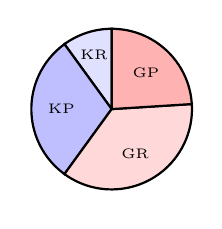
\begin{tikzpicture}[scale=0.85]
  \draw[thick, fill=blue!12] (0,0) -- (90:1.2) arc (90:126:1.2) -- cycle;
  \draw[thick, fill=blue!25] (0,0) -- (126:1.2) arc (126:234:1.2) -- cycle;
  \draw[thick, fill=red!15] (0,0) -- (234:1.2) arc (234:363.6:1.2) -- cycle;
  \draw[thick, fill=red!30] (0,0) -- (3.6:1.2) arc (3.6:90:1.2) -- cycle;
  \node[font=\tiny] at (108:0.85) {KR};
  \node[font=\tiny] at (180:0.75) {KP};
  \node[font=\tiny] at (298:0.75) {GR};
  \node[font=\tiny] at (47:0.75) {GP};
\end{tikzpicture}
\end{column}
\begin{column}{0.48\textwidth}
\textbf{Behavioral strategy}
\begin{itemize}
    \item At each information set, when you get there: flip that set's coin
    \item One coin per information set
\end{itemize}
\bsk
\centering
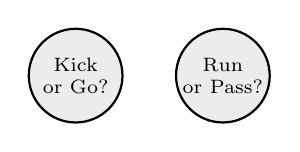
\begin{tikzpicture}[scale=0.85]
  \draw[thick, fill=gray!15] (0,0) circle (0.7);
  \node[font=\scriptsize, align=center] at (0,0) {Kick\\or Go?};
  \draw[thick, fill=gray!15] (2.2,0) circle (0.7);
  \node[font=\scriptsize, align=center] at (2.2,0) {Run\\or Pass?};
\end{tikzpicture}
\end{column}
\end{columns}
\bsk
OSU behavioral: \ $\beh[cc|cc]{\text{Kick} & \text{Go} & \text{Run} & \text{Pass}}{p & 1-p & q & 1-q}$ \quad Needs \underline{\hspace{0.4in}} numbers
\vspace{-0.3in}
\end{frame}

\begin{frame}{Formal Definition: Behavioral Strategy}
\begin{block}{Definition (Bonanno 7.1.1)}
A \textbf{behavioral strategy} for a player is a list of probability distributions, one for every information set of that player. Each one is over the choices at that information set.
\end{block}
\bsk
How many numbers? \ Ex: 3 information sets, 2 choices at each
\begin{itemize}
    \item Pure strategies: \underline{\hspace{0.4in}}
    \item Mixed strategy: \underline{\hspace{0.4in}} numbers
    \item Behavioral strategy: \underline{\hspace{0.4in}} numbers
\end{itemize}
\bsk
\onslide<2->{\textbf{Fact:} Mixed grows by \textbf{multiplying}, behavioral grows by \textbf{adding}}
\vfill
\onslide<3->{\textbf{Fact:} One information set? Then mixed $=$ behavioral (like Michigan)}
\vspace{-0.3in}
\end{frame}

\begin{frame}{Are They the Same?}
Suppose OSU's coach uses this mixed strategy:
$$\sigma_{OSU}=\begin{pmatrix} (\text{Kick},\text{Run}) & (\text{Kick},\text{Pass}) & (\text{Go},\text{Run}) & (\text{Go},\text{Pass}) \\ 0.1 & 0.3 & 0.36 & 0.24\end{pmatrix}$$
\bsk
Find a behavioral strategy that does the same thing:
\bsk
Pr(Go) $=$ \underline{\hspace{1.8in}}
\bsk
Pr(Run $\mid$ Go) $=$ \underline{\hspace{1.8in}}
\bsk
\onslide<2->{Check: Pr(Go and Run) $=$ \underline{\hspace{1.2in}} \ $=0.36$ \ \checkmark}
\vfill
\onslide<3->{\textbf{Lesson:} The 0.1 vs.\ 0.3 split never matters. Many mixed strategies $\to$ one behavioral}
\vspace{-0.3in}
\end{frame}

\begin{frame}{Kuhn's Theorem}
\begin{block}{Theorem (Kuhn, 1953)}
In games with \textbf{perfect recall}, for every mixed strategy there is a behavioral strategy that gives the same probability over terminal nodes
\end{block}
\bsk
(No matter what the other players do)
\bsk
\textbf{Thus:} Use behavioral strategies. Simpler, and nothing is lost
\bsk
Recall perfect recall (Chapter 4):
\begin{itemize}
    \item Never forget what you knew
    \item Never forget what you did
\end{itemize}
\vfill
{\footnotesize Bonanno works through his own example (Figure 7.3) on pp.~239--241.}
\vspace{-0.2in}
\end{frame}

\begin{frame}{Without Perfect Recall}
\begin{columns}[T]
\begin{column}{0.42\textwidth}
\centering
\begin{gametree}[player names={1}, scale=0.8]
  \branch[player=1, root=w, label=90] from (0,0) to[v=1.4, h=4.4] {a; b};
  \branch[player=1, label=none] from (w1) to[v=1.4, h=1.8] {c($z_1$); d($z_2$)};
  \branch[label=none] from (w2) to {c($z_3$); d($z_4$)};
  \informset (w1) -- (w2);
\end{gametree}
\bsk
\raggedright
P1 forgets whether they chose $a$ or $b$
\end{column}
\begin{column}{0.56\textwidth}
Mixed: \ $\begin{pmatrix} (a,c) & (a,d) & (b,c) & (b,d) \\ \tfrac12 & 0 & 0 & \tfrac12\end{pmatrix}$
\bsk
Gives \ $z_1$: $\tfrac12$, \ $z_4$: $\tfrac12$
\bsk
Behavioral: \ $\beh[cc|cc]{a & b & c & d}{p & 1-p & q & 1-q}$
\bsk
Need $\Pr(z_2)=$ \underline{\hspace{0.7in}} $=0$
\bsk
\onslide<2->{$\Rightarrow p=0$ \ or \ $q=1$\\[4pt]
$\Rightarrow \Pr(z_1)=0$ \ or \ $\Pr(z_4)=0$}
\bsk
\onslide<3->{Can't be done!}
\end{column}
\end{columns}
\vfill
\onslide<4->{\textbf{Ex:} ``Player 1'' is a team that can't talk once play starts. A pre-game coin flip keeps them coordinated. Separate coin flips can't (not in the book)}
\vspace{-0.3in}
\end{frame}

\begin{frame}{Two Ways To Be Unpredictable}
Randomize \textbf{as you go} (behavioral):
\begin{itemize}
    \item \textbf{Play-calling}: each down, run or pass?
    \item \textbf{Pitching}: each pitch, fastball or curveball?
    \item \textbf{Poker}: each betting round, bluff or fold?
    \item \textbf{Penalty kicks}: each kick, left or right?
\end{itemize}
\bsk
Randomize \textbf{a whole plan in advance} (mixed):
\begin{itemize}
    \item \textbf{Security}: LAX's ARMOR software draws each day's checkpoint schedule
    \item \textbf{Inspections}: random drug-test lists, tax audits, restaurant inspections
    \item \textbf{Exams}: a random version of the test, handed out before it starts
\end{itemize}
\bsk
Kuhn: with perfect recall, the two are equally powerful
\vfill
{\footnotesize Not in the book. ARMOR: Pita et al.\ (2008, AAMAS).}
\vspace{-0.2in}
\end{frame}

\begin{frame}{But Those Are More Complicated}
Real versions add:
\begin{itemize}
    \item Many information sets, many choices at each
    \item Opponents who learn from what you did earlier
    \item Organizations that \textbf{forget}: no perfect recall!
    \begin{itemize}
        \item New staff, lost notes, no one knows last week's schedule
    \end{itemize}
\end{itemize}
\bsk
Core idea survives: one coin at each decision point is enough, \textbf{if} you remember
\vfill
\vspace{-0.4in}
\end{frame}

% ==============================================================
% BIGGER EXAMPLE: BONANNO FIGURES 7.7 - 7.11
% ==============================================================
% Payoffs are (P1, P2, P3). Colors remapped for the P2-vs-P3 matrices as
% in deck 06.
% ---------------------------------------------------------------------

\begin{frame}[standout]
A Bigger Example
\end{frame}

\begin{frame}{Figure 7.7}
Find the SPNE
\bsk
\centering
\begin{gametree}[player names={1, 2, 3}, scale=1.08]
  \figsevenseven
\end{gametree}
\bsk
\raggedright
How many proper subgames? \underline{\hspace{0.6in}} \ Any pure NE in them?
\vspace{-0.3in}
\end{frame}

\begin{frame}{Figure 7.8: The Left Subgame}
\begin{columns}[c]
    \begin{column}{0.45\textwidth}
        \centering
        {\colorlet{pA}{player2}\colorlet{pB}{player3}\colorlet{player1}{pA}\colorlet{player2}{pB}%
        \begin{gametree}[player names={2, 3}]
          \branch[player=1, root=w, label=90] from (0,0) to[v=1.4, h=3.2] {A; B};
          \branch[player=2, label=none] from (w1) to[v=1.6, h=1.5] {C(3,1); D(0,2)};
          \branch[label=none] from (w2) to {C(0,3); D(1,2)};
          \informset[player=2] (w1) -- (w2);
        \end{gametree}}
    \end{column}
    \begin{column}{0.53\textwidth}
        \centering
        {\colorlet{pA}{player2}\colorlet{pB}{player3}\colorlet{player1}{pA}\colorlet{player2}{pB}%
        \begin{matrixgame}[top={C, D}, left={A, B}, player names={Player 2, Player 3}]
          \payoffmatrix{3,1 & 0,2 \\ 0,3 & 1,2}
        \end{matrixgame}}
    \end{column}
\end{columns}
\bsk
$q=\Pr(C)$ makes P2 indifferent: \hspace{1.2in} $p=\Pr(A)$ makes P3 indifferent:
\vspace{0.5in}

Payoffs (P1, P2, P3): \ (\underline{\hspace{0.5in}}, \underline{\hspace{0.5in}}, \underline{\hspace{0.5in}}) \hfill {\footnotesize P1's payoffs come from the tree}
\vspace{-0.3in}
\end{frame}

\begin{frame}{Figure 7.10: The Right Subgame}
\begin{columns}[c]
    \begin{column}{0.45\textwidth}
        \centering
        {\colorlet{pA}{player2}\colorlet{pB}{player3}\colorlet{player1}{pA}\colorlet{player2}{pB}%
        \begin{gametree}[player names={2, 3}]
          \branch[player=1, root=w, label=90] from (0,0) to[v=1.4, h=3.2] {E; F};
          \branch[player=2, label=none] from (w1) to[v=1.6, h=1.5] {G(0,3); H(1,2)};
          \branch[label=none] from (w2) to {G(2,1); H(0,3)};
          \informset[player=2] (w1) -- (w2);
        \end{gametree}}
    \end{column}
    \begin{column}{0.53\textwidth}
        \centering
        {\colorlet{pA}{player2}\colorlet{pB}{player3}\colorlet{player1}{pA}\colorlet{player2}{pB}%
        \begin{matrixgame}[top={G, H}, left={E, F}, player names={Player 2, Player 3}]
          \payoffmatrix{0,3 & 1,2 \\ 2,1 & 0,3}
        \end{matrixgame}}
    \end{column}
\end{columns}
\bsk
$q=\Pr(G)$ makes P2 indifferent: \hspace{1.2in} $p=\Pr(E)$ makes P3 indifferent:
\vspace{0.5in}

Payoffs (P1, P2, P3): \ (\underline{\hspace{0.5in}}, \underline{\hspace{0.5in}}, \underline{\hspace{0.5in}})
\vspace{-0.3in}
\end{frame}

\begin{frame}{Figure 7.11: What's Left}
\centering
\begin{gametree}[player names={1, 2, 3}, scale=1.0]
  \branch[player=1, root=w, label=90] from (0,0) to[v=1.5, h=6.0] {L(1.125,0.75,2); R(1,0.67,2.33)};
\end{gametree}
\bsk
\raggedright
Player 1 chooses: \underline{\hspace{0.6in}}
\bsk
\textbf{SPNE}, in behavioral strategies:
\bsk
\centering
P1: $\beh{L & R}{\underline{\hspace{0.25in}} & \underline{\hspace{0.25in}}}$
\qquad
P2: $\beh[cc|cc]{A & B & E & F}{\underline{\hspace{0.25in}} & \underline{\hspace{0.25in}} & \underline{\hspace{0.25in}} & \underline{\hspace{0.25in}}}$
\\[10pt]
P3: $\beh[cc|cc]{C & D & G & H}{\underline{\hspace{0.25in}} & \underline{\hspace{0.25in}} & \underline{\hspace{0.25in}} & \underline{\hspace{0.25in}}}$
\vspace{-0.3in}
\end{frame}

% ==============================================================
% 7.3 PROBLEMS WITH SUBGAME-PERFECT EQUILIBRIUM
% ==============================================================

\begin{frame}[standout]
What SPNE Gets Wrong
\end{frame}

\begin{frame}{Selten's Horse}
\begin{columns}[c]
\begin{column}{0.5\textwidth}
\centering
\horse
\end{column}
\begin{column}{0.48\textwidth}
Proper subgames? \underline{\hspace{0.6in}}
\bsk
\onslide<2->{So SPNE $=$ NE}
\bsk
\onslide<3->{Pure NE:\\[6pt]
\underline{\hspace{0.8in}} \quad \underline{\hspace{0.8in}}\\[10pt]
\underline{\hspace{0.8in}} \quad \underline{\hspace{0.8in}}}
\bsk
\onslide<4->{Are they all reasonable???}
\end{column}
\end{columns}
\vfill
{\footnotesize Bonanno Figure 7.12. Named by Selten (1975) for its shape.}
\vspace{-0.2in}
\end{frame}

\begin{frame}{Problem 1: $(a,f,c)$}
\begin{columns}[c]
\begin{column}{0.5\textwidth}
\centering
\horse
\end{column}
\begin{column}{0.48\textwidth}
P1 plays $a$. \ P2 never moves
\bsk
So P2's plan $f$ costs P2 nothing
\bsk
\onslide<2->{But \textbf{if} P2 had to move?\\[4pt]
$e$ gives \underline{\hspace{0.4in}} \quad $f$ gives \underline{\hspace{0.4in}}}
\bsk
\onslide<3->{$f$ is a bad plan. SPNE doesn't notice}
\end{column}
\end{columns}
\vspace{-0.3in}
\end{frame}

\begin{frame}{Problem 2: $(b,f,d)$}
\begin{columns}[c]
\begin{column}{0.5\textwidth}
\centering
\horse
\end{column}
\begin{column}{0.48\textwidth}
P1 plays $b$, P2 plays $f$. \ P3 never moves
\bsk
\onslide<2->{But \textbf{if} P3 had to move?\\[4pt]
Left node: $c$ \underline{\hspace{0.3in}} vs.\ $d$ \underline{\hspace{0.3in}}\\[4pt]
Right node: $c$ \underline{\hspace{0.3in}} vs.\ $d$ \underline{\hspace{0.3in}}}
\bsk
\onslide<3->{$d$ is \textbf{strictly dominated} at P3's infoset!}
\end{column}
\end{columns}
\bsk
\onslide<4->{\textbf{Lesson:} $d$ is dominated as a \textbf{choice}, not as a \textbf{strategy}\\
Unreached infosets escape the test}
\vfill
{\footnotesize Bonanno typo, p.~249: for $(b,f,d)$ it says ``Player 1 plays $a$''. Should be $b$.}
\vspace{-0.2in}
\end{frame}

\begin{frame}{So What's Missing?}
SPNE checks for rationality only in \textbf{subgames}
\begin{itemize}
    \item A subgame can't cut an information set
    \item So choices at big infosets are only checked if they're on the path of play
\end{itemize}
\bsk
The fix: Every choice should be sensible, \textbf{even off the path of play}
\begin{itemize}
    \item P3 doesn't know which node she's at\\
    $\Rightarrow$ she needs a \textbf{belief} about where she is
\end{itemize}
\bsk
\textbf{Thus:} \ $\{\text{better equilibria}\}\subseteq SPNE\subseteq NE$
\vfill
{\footnotesize Bonanno Part IV (Chapters 11--13): weak sequential, sequential, and perfect Bayesian equilibrium.}
\vspace{-0.2in}
\end{frame}

% ==============================================================
% WORKED EXAMPLE
% ==============================================================
% Deck 08's Gameday Parking game becomes the subgame after Drive.
% Answers are in the header comment.
% ---------------------------------------------------------------------

\begin{frame}[standout]
Let's Work One Out
\end{frame}

\begin{frame}{Gameday Parking, Part 2}
Jordan first decides how to get to the game:
\begin{itemize}
    \item \textbf{Bus} (COTA): on time with chance $\tfrac34$ (payoff 2), else late (payoff 0)
    \item \textbf{Drive}: then Chapter 6's parking game. CampusParc can't see where Jordan parked
\end{itemize}
\bsk
\centering
\begin{gametree}[player names={Jordan, CampusParc}, scale=0.74]
  \branch[player=1, root=w, label=90] from (-1.5,0) to[v=1.1, h=7.0] {Bus; Drive};
  \branch[player=0, label=150] from (w1) to[v=1.5, h=2.0] {$\frac34$(2,0); $\frac14$(0,0)};
  \branch[player=1, label=30] from (w2) to[v=1.3, h=3.4] {Pay; West; Neil};
  \branch[player=2, label=none] from (w21) to[v=1.6, h=1.5] {PW(1,0); PN(1,0)};
  \branch[label=none] from (w22) to {PW(0,2); PN(4,0)};
  \branch[label=none] from (w23) to {PW(3,0); PN(0,1)};
  \informset[label=none] (w21) -- (w23);
  \node[text=player2, anchor=west, font=\small] at ($(w23)+(0.45,0)$) {CampusParc};
\end{gametree}
\vspace{-0.3in}
\end{frame}

\begin{frame}{Gameday Parking, Part 2}
\begin{enumerate}
    \item List Jordan's pure strategies. How many numbers for a mixed strategy? A behavioral one? \vspace{0.3in}
    \item What is Jordan's expected payoff from Bus? \vspace{0.25in}
    \item Solve the parking subgame (recall Chapter 6). Payoffs? \vspace{0.35in}
    \item Find the SPNE. Write it in behavioral strategies \vspace{0.35in}
    \item How reliable must the bus be before Jordan takes it? \vspace{0.25in}
\end{enumerate}
\end{frame}

\begin{frame}{What Have We Learned, Charlie Brown?}
\begin{itemize}
    \item Nature in a tree? Replace the lottery with its \textbf{expected utility}
    \item \textbf{Behavioral strategy}: one probability distribution per information set
    \begin{itemize}
        \item Mixed: spin one wheel over whole plans. Behavioral: flip as you go
    \end{itemize}
    \item \textbf{Kuhn (1953)}: with perfect recall, behavioral $=$ mixed
    \item \textbf{Selten (1965)}: with cardinal payoffs, a SPNE always exists
    \begin{itemize}
        \item Solve subgames with mixed NE when there's no pure one
    \end{itemize}
    \item SPNE can still allow silly choices at unreached infosets (Selten's horse)
\end{itemize}
\vfill
\vspace{-0.4in}
\end{frame}

\begin{frame}{Reading \& Practice}
\begin{itemize}
    \item Bonanno, \textit{Game Theory}, Chapter 7
    \begin{itemize}
        \item \S7.1: read for behavioral strategies and Kuhn's theorem.\\
        Skim the formal ``game with cardinal payoffs'' part
        \item \S7.2--7.3: read carefully
    \end{itemize}
    \item Exercises: \S7.4.1 (7.1, 7.2, 7.3), \S7.4.2 (7.5, 7.7)
    \begin{itemize}
        \item 7.4 and 7.6 review Chapter 5's utility calibration
        \item 7.8 is harder. 7.9 (the mugger) is a challenge
    \end{itemize}
    \item Solutions in \S7.5. Try them first
\end{itemize}
\vfill
\end{frame}

\end{document}
